% !TEX root =  ../STVR-model-seeding.tex

%%%%%%%%%%%%%%%%%%%%%%
 \section{Behavioral Model and Test Seeding for Crash Reproduction}
 \label{sec:model_seeding:approach}
 %%%%%%%%%%%%%%%%%%%%%%

The goal of behavioral model seeding (denoted model seeding hereafter) is to abstract the behavior of the software under test using models and use that abstraction during the search. At the unit test level (which is the considered test generation level in this study), each model is a transition system, like in Figure \ref{fig:list}, and represents possible usages of a class: \ie possible sequences of method calls observed for objects of that class.

\begin{figure*}[t]
    \centering
    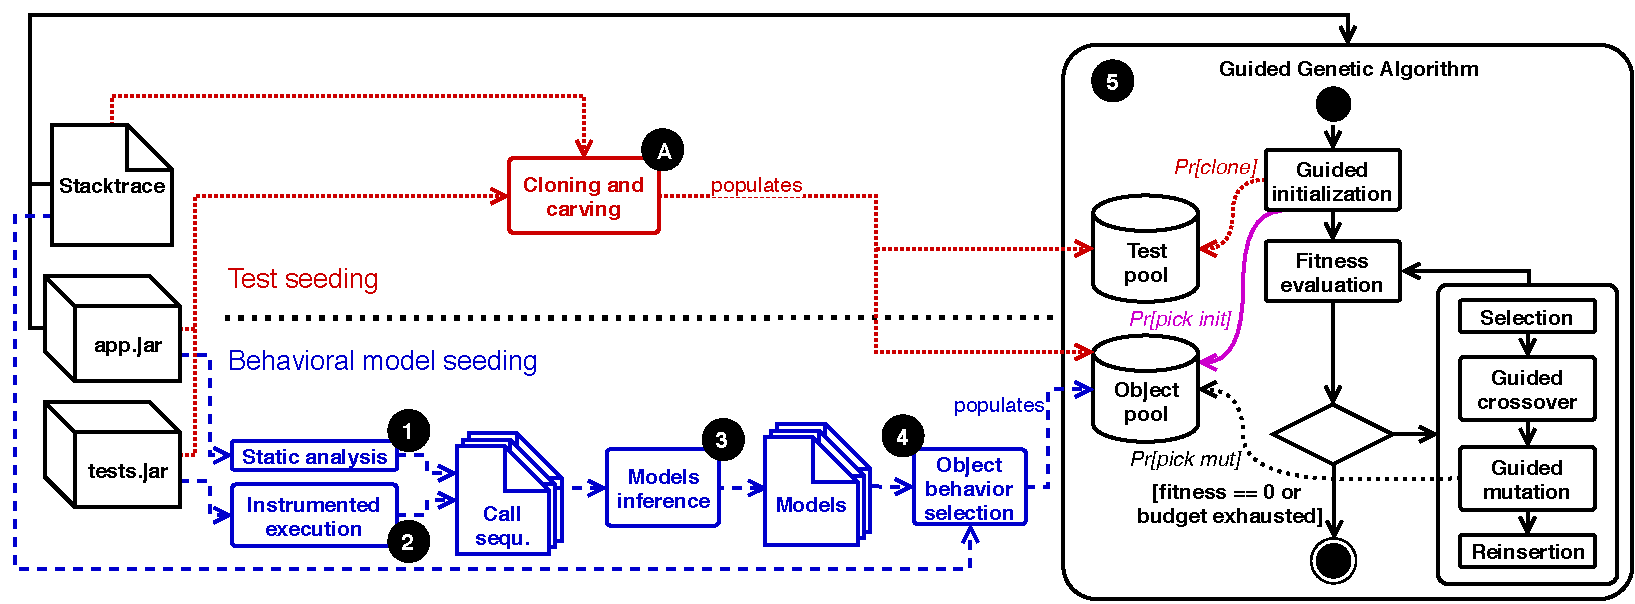
\includegraphics[width=\textwidth]{papers/model_seeding/figures/implementation/approach.pdf}
%    \vspace{-1mm}
    \caption{General overview of model seeding and test seeding for search-based crash reproduction}
    \label{fig:approach}
%    \vspace{-3mm}
\end{figure*}

The main steps of our model seeding approach, presented in Figure~\ref{fig:approach}, are:
 the \emph{inference} of the individual models \circled{3} (described in Section \ref{ssec:inference}) from the \emph{call sequences} collected through \emph{static analysis} \circled{1} performed on the application code (described in Section \ref{ssec:staticanalysis}), and \emph{dynamic analysis} \circled{2} of the test cases (described in Section \ref{ssec:dynamicanalysis});
 and for each model, the \emph{selection of abstract object behaviors} \circled{4}, that are concretized into Java objects  (described in Section \ref{ssec:abstract-selection}), stored in an \emph{object pool} from which the guided genetic algorithm \circled{5}  (described in Section \ref{ssec:gga}) can randomly pick objects to build test cases during the search process.

%--------------------------------
\subsection{Model inference}
\label{ssec:inference}
%--------------------------------

Call sequences are obtained by using static analysis on the bytecode of the application \circled{1} and by instrumenting and executing the existing test cases \circled{2}.

We use $n$-gram inference to build the transition systems used for model seeding. $N$-gram inference takes a set of sequences of actions as input to produce a transition system where the $n^{th}$ action depends on the $n-1$ previously executed actions.

%For  $2$-gram inference, the next action to execute only depends on the current state in the transition system. 

A large value of $n$ for the $n$-gram inference would result in wider transition systems with more states and less incoming transitions, representing a more constrained behavior and producing less diverse test cases. In contrast, a small  value of $n$ enables better diversity in the behavior allowed by the model (ending up in more diverse abstract object behaviors), requires less observations to reach stability of the model, simplifies the inference, and results in a more compact model~\cite{Sprenkle2013,Sprenkle2011a}.  For these reasons, we use $2$-gram inference to build our models. % used for model seeding.
%
%For instance, the transition system model in Figure~\ref{fig:list} has been partially generated from the following call sequences collected from the code and the test cases:
%
%{\ttfamily\footnotesize<size(), re\-move(), add(Ob\-ject), size(), size(), size(), get(), re\-move(), add(Ob\-ject)>};
%{\ttfamily\footnotesize<i\-te\-ra\-tor(),add(Ob\-ject)>}; \etc.
%
%Each transition in Figure~\ref{fig:list} corresponds to a method call in one of the sequences, and for each sequence, there exists a path in the model. % corresponding to that sequence.

%\andy{Should this choice for static and dynamic be better argumented? Why not use static for the test case as well?
%\pouria{I have tried to answer this question in subsection 4.1.2. We can move the answer here}
%}
%
For each class, the model \circled{3} is obtained using a  $2$-gram inference method using the call sequences of that class.

%
For instance, in the transition system of Figure \ref{fig:list}, the action \texttt{size()}, executed from state $s_3$ at step $k$ only depends on the fact that the action \texttt{add(Object)} has been executed at step $k-1$, independently of the fact that there is a step $k-2$ during which the action \texttt{iterator()} has been executed.

Calls to constructors are considered as method calls during model inference. However, constructors may not appear in any transition of the model if no constructor call was observed during the collection of the call sequences.  This is usually the case when the call sequences used to infer the model have been captured from objects that are parameters or attributes of a class. If an abstract object behavior does not start by a call to a constructor, a constructor is randomly chosen to initialize the object during the concretization.

% The model inference is a one time task. If any class changes in the future implementations, an extra analysis of the changed class will update the models.

For one version of the software under test, the model inference is a one time task. Models can then be directly reused for various crash reproductions.

\subsubsection{Static analysis of the application}
\label{ssec:staticanalysis}

The static analysis is performed on the bytecode of the application. We apply this analysis to all of the available classes in the software under test.  In each method of these classes, we build the control flow graph, and for each object of that method, we collect the sequences of method calls on that object.
For each object, each path in the control flow graph will correspond to one sequence of method calls. For instance, if the code contains an \texttt{if-then-else} statement, the \texttt{true} and \texttt{false} branches will produce two call sequences. In the case of a loop statement, the  \texttt{true} branch is considered only once. The static analysis is \emph{intraprocedural}, meaning that only the calls in the current method are considered. If an object is passed as a parameter of a call to a method that (internally) calls other methods on that object, those internal calls will not appear in the call sequences.
This analysis ensures collecting all of the existing relevant call sequences for any internal or external class, which is used in the project.

%The static analysis is performed on the bytecode of the application. To keep the process within a reasonable amount of time, we only apply this analysis to the classes involved in the stack trace.  In each method of these classes, we collect the sequences of method calls for all of the \andy{Should it be ``available'' or ``involved''?} \andy{Other question could be: how big is the gain in efficiency of the on-demand solution versus the ``do everything'' solution?} available classes. Since a stack trace represents a call hierarchy, this analysis ensures collecting relevant call sequences for at least the class at frame level $k$ in the methods of the class at frame level $k+1$. For instance, in the stack trace of Listing \ref{lst:model_seeding:stacktrace}, call sequences of \texttt{BaseObject} objects are collected (at least) in class \texttt{XWikiDocument}, which calls methods of  \texttt{BaseObject}.

\subsubsection{Dynamic analysis for the test cases}
\label{ssec:dynamicanalysis}

Since the existing manually developed test cases exemplify potential usage scenarios of the software under test, we apply dynamic analysis to collect all of the transpired sequences during the execution of these scenarios. Contrarily to static analysis, which would require an expensive effort and produce imprecise call sequences, dynamic analysis is \emph{interprocedural}. Meaning that the sequences include calls appearing in the test cases, but also internal calls triggered by the execution of the test case (\eg if the object is passed as a parameter to a method and methods are internally called on that object ). Hence, through dynamic analysis, we gain a more accurate insight into the class usages in these scenarios.

Dynamic analysis of the existing tests is done in a similar way to the carving approach of Rojas \etal~\cite{Rojas2016}: instrumentation adds log messages to indicate when a method is called, and the sequences of method calls are collected after execution. In similar fashion to static analysis, we collect call sequences of any observed object (even objects which are not defined in the software under test).
The representativeness of the collected sequences depends on the coverage of the existing tests.

%\andy{If this is still relevant, this MSc thesis shows that $\sim$80 of jUnit tests are actually integration tests. See my mattermost message Xavier...}
%\andy{I don't exactly know what you want... this article says that private methods are often tested indirectly. Is that what you are after?  (A Simple and Practical Approach to Unit Testing: The JML and JUnit Way, ECOOP 2002)}


%---------------------------------------------
\subsection{Abstract Object Behaviors Selection}
\label{ssec:abstract-selection}
%---------------------------------------------

Abstract object behaviors are selected from the transition systems and concretized to populate the object pool used during the search.
%
To limit the number of objects in the pool, we only select abstract object behaviors from two categories of models:  models of internal classes (\ie classes belonging to packages of the software under test) and models of dependency classes (\ie classes belonging to packages of external dependencies) that are involved in the stack trace.
Since we do not seek to validate the implementation of the application, the states are ignored during the selection process.

\subsubsection{Selection}
\label{ssec:selection}

There exist various criteria to select abstract object behaviors from transition systems~\cite{Utting2007}.
%
To successfully guide the search, we need to establish a good ratio between \emph{exploration} (the ability to visit new regions of the search space) and \emph{exploitation} (the ability to visit the neighborhood of previously visited regions) \cite{vcrepinvsek2013}.
The guided genetic operators which are introduced in the \evocrash approach \cite{soltani2017} guarantee the exploitation by focusing the search based on the methods in the stack trace. However, depending on the stack trace, focusing on particular methods may reduce the exploration. Poor exploration decreases the diversity of the generated tests and may trap the search process in local optima.

To improve the exploration ability in the search process, we use \emph{dissimilarity} as the criterion to select the abstract object behaviors. Compared to classical structural coverage criteria that seek to cover as many parts of the transition system as possible, dissimilarity tries to increase diversity among the test cases by maximizing a distance $d$ (\ie the Jaccard index \cite{Jaccard1901}):
$$
d = 1 - \frac{ \{call_{1i} \in b_{1}\} \cap \{call_{2j} \in b_{2}\}}{\{call_{1i} \in b_{1}\} \cup \{call_{2j} \in b_{2}\}}
$$
Where $b_{1} = <\mathit{call}_{11}, \mathit{call}_{12}, \ldots> $ and $ b_{2} = <\mathit{call}_{21}, \mathit{call}_{22}, \ldots>$ are two abstract object behaviors.

\subsubsection{Concretization}
\label{ssec:concretization}

Each abstract object behavior has to be concretized to an object and method calls before being added to the objects pool. In other words, for each abstract object behavior, if the constructor invocation is not the first action, one constructor is randomly called; and the methods are called on this object in the order specified by the abstract object behavior with randomly generated parameter values. Due to the randomness, each concretization may be different from the previous one. For each abstract object behavior, $n$ concretizations (default value is $n=1$  to balance scalability and diversity of the objects in the object pool) are done for each abstract object behavior and saved in the object pool.
%
For instance, Listing \ref{lst:concretized-test} shows the concretized abstract object behavior {\ttfamily\footnotesize <add(Object), add(Object)>} derived from the transition system model of Figure \ref{fig:list}. The type of the parameters (\texttt{EuclideanIntegerPoint}) is randomly selected during the concretization and created with required parameter values (an integer array here).


\begin{lstlisting}[
language=Java,
caption={Concretized abstract object behavior for \texttt{LinkedList} based on the transition system model of Figure \ref{fig:list}},
label=lst:concretized-test,
float=t]
int[] t = new int[7];
t[3] = -2147483647;
EuclideanIntegerPoint ep = new EuclideanIntegerPoint(t);
LinkedList<[...]> lst = new LinkedList<>();
lst.add(ep);
lst.add(ep);
\end{lstlisting}


%----------------------------------------------------------
\subsection{Guided Initialization and Guided Mutation}
\label{ssec:gga}
%----------------------------------------------------------

Classes are instantiated to create objects during two main steps of the guided genetic algorithm: guided initialization, where objects are needed to create the initial set of test cases; and guided mutation, where objects may be required as parameters when adding a method call. When no seeding is used, those objects are randomly created (as in the concretization step described in Section~\ref{ssec:concretization}) by calling the constructor and random methods.

Finally, to preserve exploration in model seeding, objects are picked from the object pool during guided initialization (resp. guided mutation) according to a user-defined probability $Pr[pick\ init]$ (resp. $Pr[pick\ mut]$), and randomly generated otherwise.
In our evaluation, we considered four different values for $Pr[pick\ init] \in \{0.2, 0.5, 0.8, 1.0\}$, to study the effect of model seeding on the initialization of the search process. Furthermore, we fixed the value of $Pr[pick\ mut] = 0.3$, corresponding to the default value of $Pr[pick\ mut]$ for test seeding for classical unit test generation in \evosuite.
%The value of the probability depends on the number and diversity of the concretized abstract object behaviors. For instance, a small model will deliver few different abstract object behaviors. In this case, lower probability values allow more randomly generated objects with calls to methods that do not appear in the model. In contrast, a large model, denoting complex behavior for the objects, may require higher probability values to avoid incorrect sequences of method invocations.



\begin{lstlisting}[
    numbers=left,
    caption={Stack trace excerpt for MATH-79b},
    label=lst:MATH-79b-trace,
    float=t]
    java.lang.NullPointerException
     at ...KMeansPlusPlusClusterer.assignPointsToClusters()
     at ...KMeansPlusPlusClusterer.cluster()
    \end{lstlisting}

\begin{lstlisting}[
language=Java,
escapechar=|,
caption={Test generated for frame 2 of MATH-79b (Listing \ref{lst:MATH-79b-trace})},
label=lst:generated-test,
float=t]
public void testCluster() throws Exception{
 int[] t = new int[7]; | \label{line:startobject} |
 t[3] = (-2147483647);
 EuclideanIntegerPoint ep = new EuclideanIntegerPoint(t);
 LinkedList<[...]> lst = new LinkedList<>();
 lst.add(ep);
 lst.add(ep); | \label{line:endobject} |
 KMeansPlusPlusClusterer<[...]> kmean = new KMeansPlusPlusClusterer<>(12);
 lst.offerFirst(ep); | \label{line:additional} |
 kmean.cluster(lst, 1, (-1357));} | \label{line:target} |
\end{lstlisting}



As an example of object picking in action, test case generation with model seeding generated the test case in Listing \ref{lst:generated-test} for the second frame of the stack trace from the crash MATH-79b from the Apache commons math project, reported in Listing \ref{lst:MATH-79b-trace}.
%
The target method is the last method called in the test (line \ref{line:target}) and throws a \texttt{NullPointerException}, reproducing the input stack trace. The first parameter of the method has to be a \texttt{Collection<T>} object. In this case, the guided genetic algorithm picked the list object from the object pool (from Listing \ref{lst:concretized-test}) and inserted it in the test case (lines \ref{line:startobject} to \ref{line:endobject}). The algorithm also modified that object (during guided mutation) by invoking an additional method on the object (line \ref{line:additional}).

%-----------------------------
 \subsection{Test Seeding}
%-----------------------------

As described in Section \ref{ssec:background:testseeding}, test seeding starts by executing the test cases (Figure \ref{fig:approach} box \circled{A}) for carving and cloning, and subsequently populating the test and object pools. Like for model seeding, only internal classes and external classes appearing in the stack trace are considered.

For crash reproduction, the test pool is used only during guided initialization to clone test cases that contain the target class, according to a user-defined $Pr[clone]$ probability. If the target method is not called in the cloned test case, the guided initialization also mutates the test case to add a call to the target method.
%
The object pool is used during the guided initialization and guided mutation to pick objects. 
As described by Rojas \etal~\cite{Rojas2016}, the properties of using the object pool during initialization ($Pr[pick\ init]$) and mutation ($Pr[pick\ mut]$) are indicated as a single property called \texttt{p\_object\_pool} in test seeding.


%------------------------------------------------------------------------
% \subsection{Comparison between behavioral model seeding and test seeding}
%------------------------------------------------------------------------

%Behavioral model seeding exploits both test cases and source code, thereby \emph{subsuming} test seeding regarding the observed behavior of the application that is reused during the search. Test seeding only uses dynamic analysis, which entails that it collects more accurate information from the potential usage scenarios of the software under test; it also means that this strategy collects more limited information for seeding. If these limited amounts of call sequences differ from the call sequences needed to reproduce the crash scenario, test seeding can misguide the crash reproduction search process.
%
%For instance, to initialize a \texttt{List} like in Listing~\ref{lst:generated-test}, test seeding can only seed the call sequences which are observed during the execution of the test cases, while model seeding can use any path in the transition system of Figure~\ref{fig:list}, which is inferred from all of the collected call sequences from static and dynamic analysis, for seeding. Using more call sequences for seeding helps behavioral model seeding to have accurate knowledge about the usage of the \texttt{List} class.
%However, by using cloning, test seeding benefits from (fixed) readily usable objects during initialization at the expense of diversity.
%\andy{mmm... what about something you also mentioned earlier... the fact that the models that come from testing are more ``precise'' and less ``open'' than those obtained statically?
%\pouria{model seeding uses the collected call sequences from both static and dynamic analysis while test seeding only uses the collected call sequences of dynamic analysis. Since more call sequences help us to have more accurate information about the class usages, we think that model seeding has more chance to cover the crash path. I tried to extend this section to explain this point more specifically. Also, I have added this discussion in the motivation section. In addition, I rephrased the section which discusses the ``precise" results of dynamic analysis (Section 4.1.2)}
%}

%Since test seeding only considers the fixed method calls sequences observed in the test cases to initialize the objects, model seeding \emph{subsumes} test seeding as it analyzes both test cases and source code for this purpose.
%In addition, even when only using the existing test cases, model seeding, which abstracts the behavior compared to test seeding,  can generate more objects with different behavior compared to test seeding.
%%
%For instance, to initialize a list like in Listing~\ref{lst:generated-test}, test seeding can only seed the call sequences which are observed during the execution of the test cases, while model seeding can use any path in the transition system of Figure~\ref{fig:list} for seeding.
